\section{Frequency mode 08}
\subsection{Spectra}
\TODO{Add FM~08 conclusions}

\begin{figure}[ht]
    \centering
    \begin{subfigure}[b]{0.9545\textwidth}
        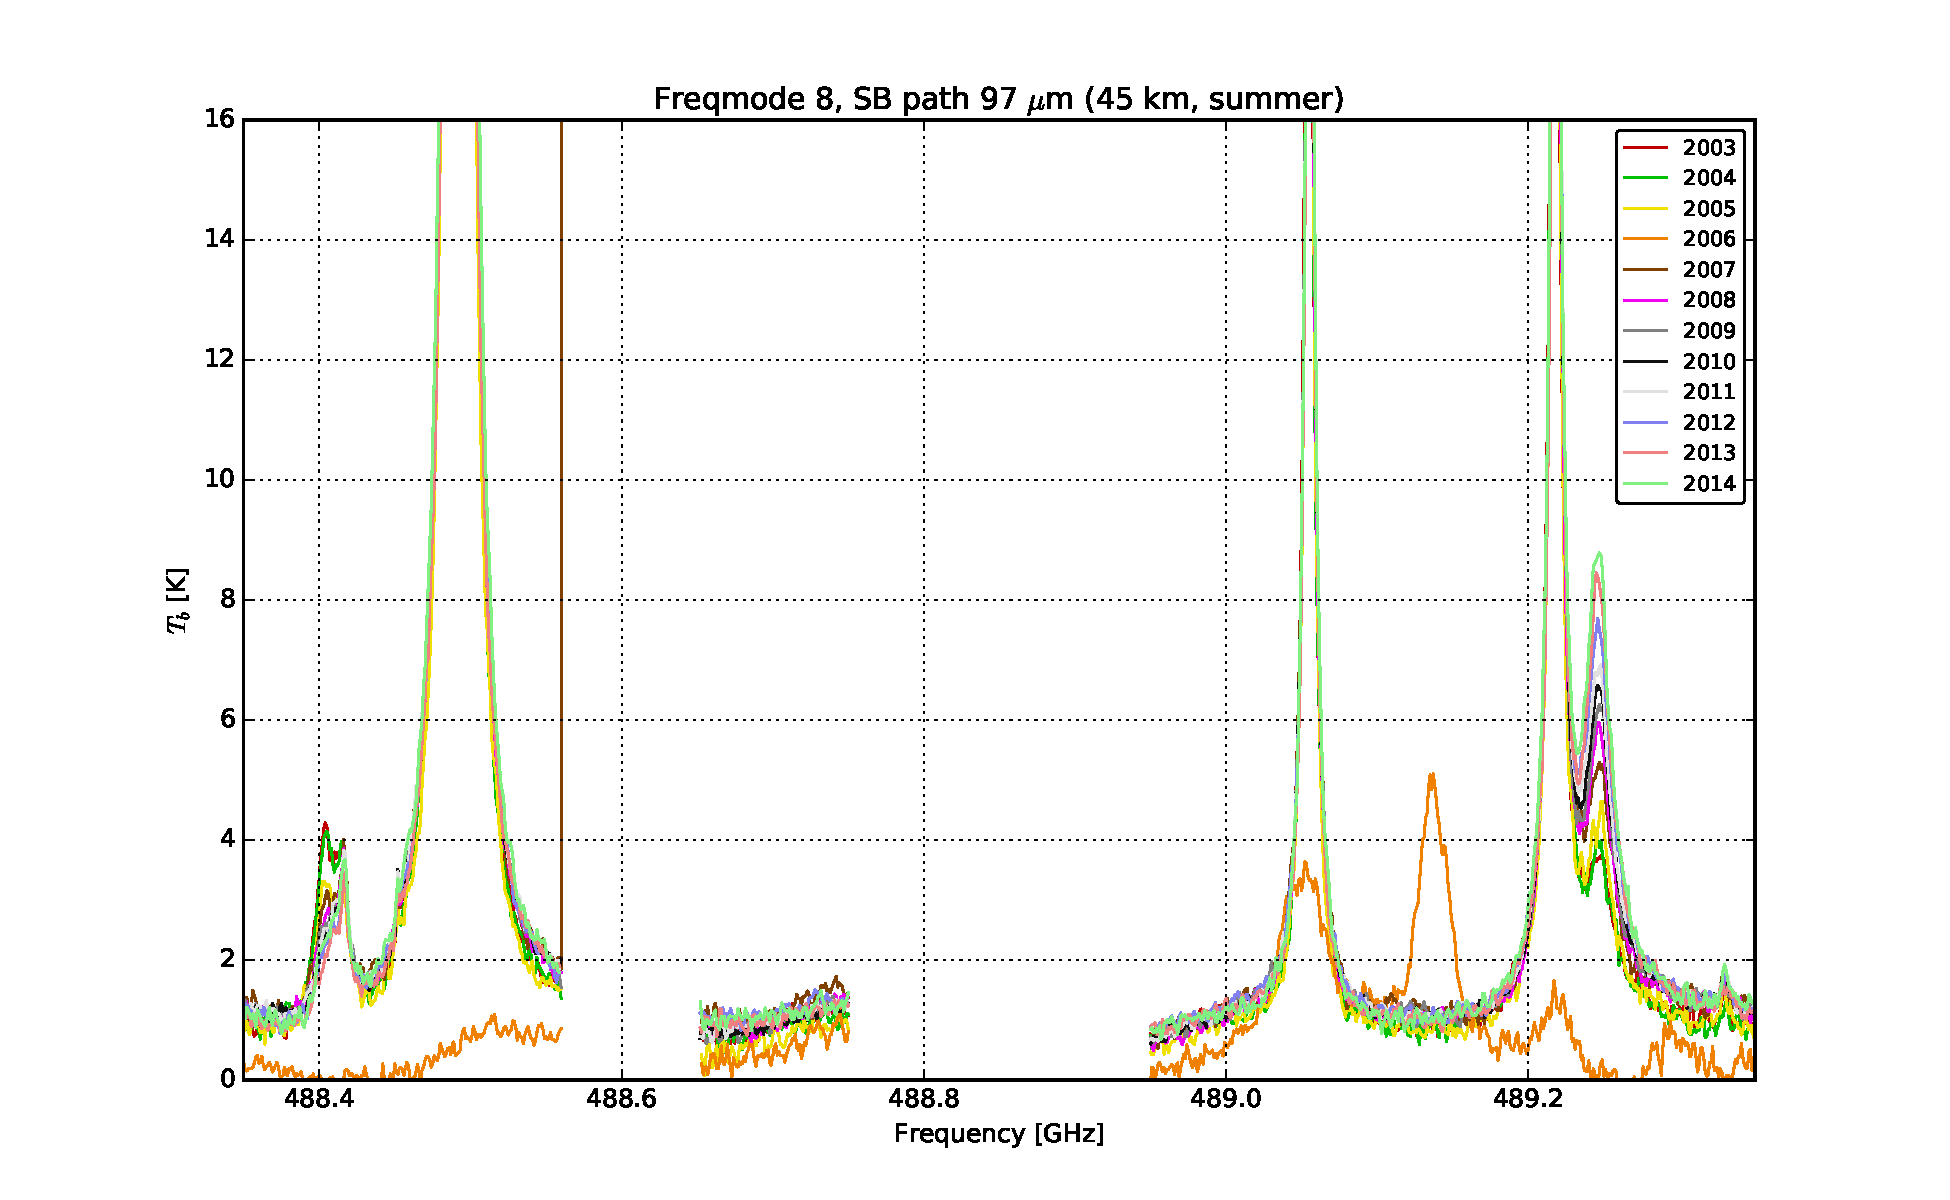
\includegraphics[width=\textwidth]{fm_08_spectra_summer_97u}
        \caption{summer}\label{fig:spectra:08:summer:97u}
    \end{subfigure}
    \begin{subfigure}[b]{0.9545\textwidth}
        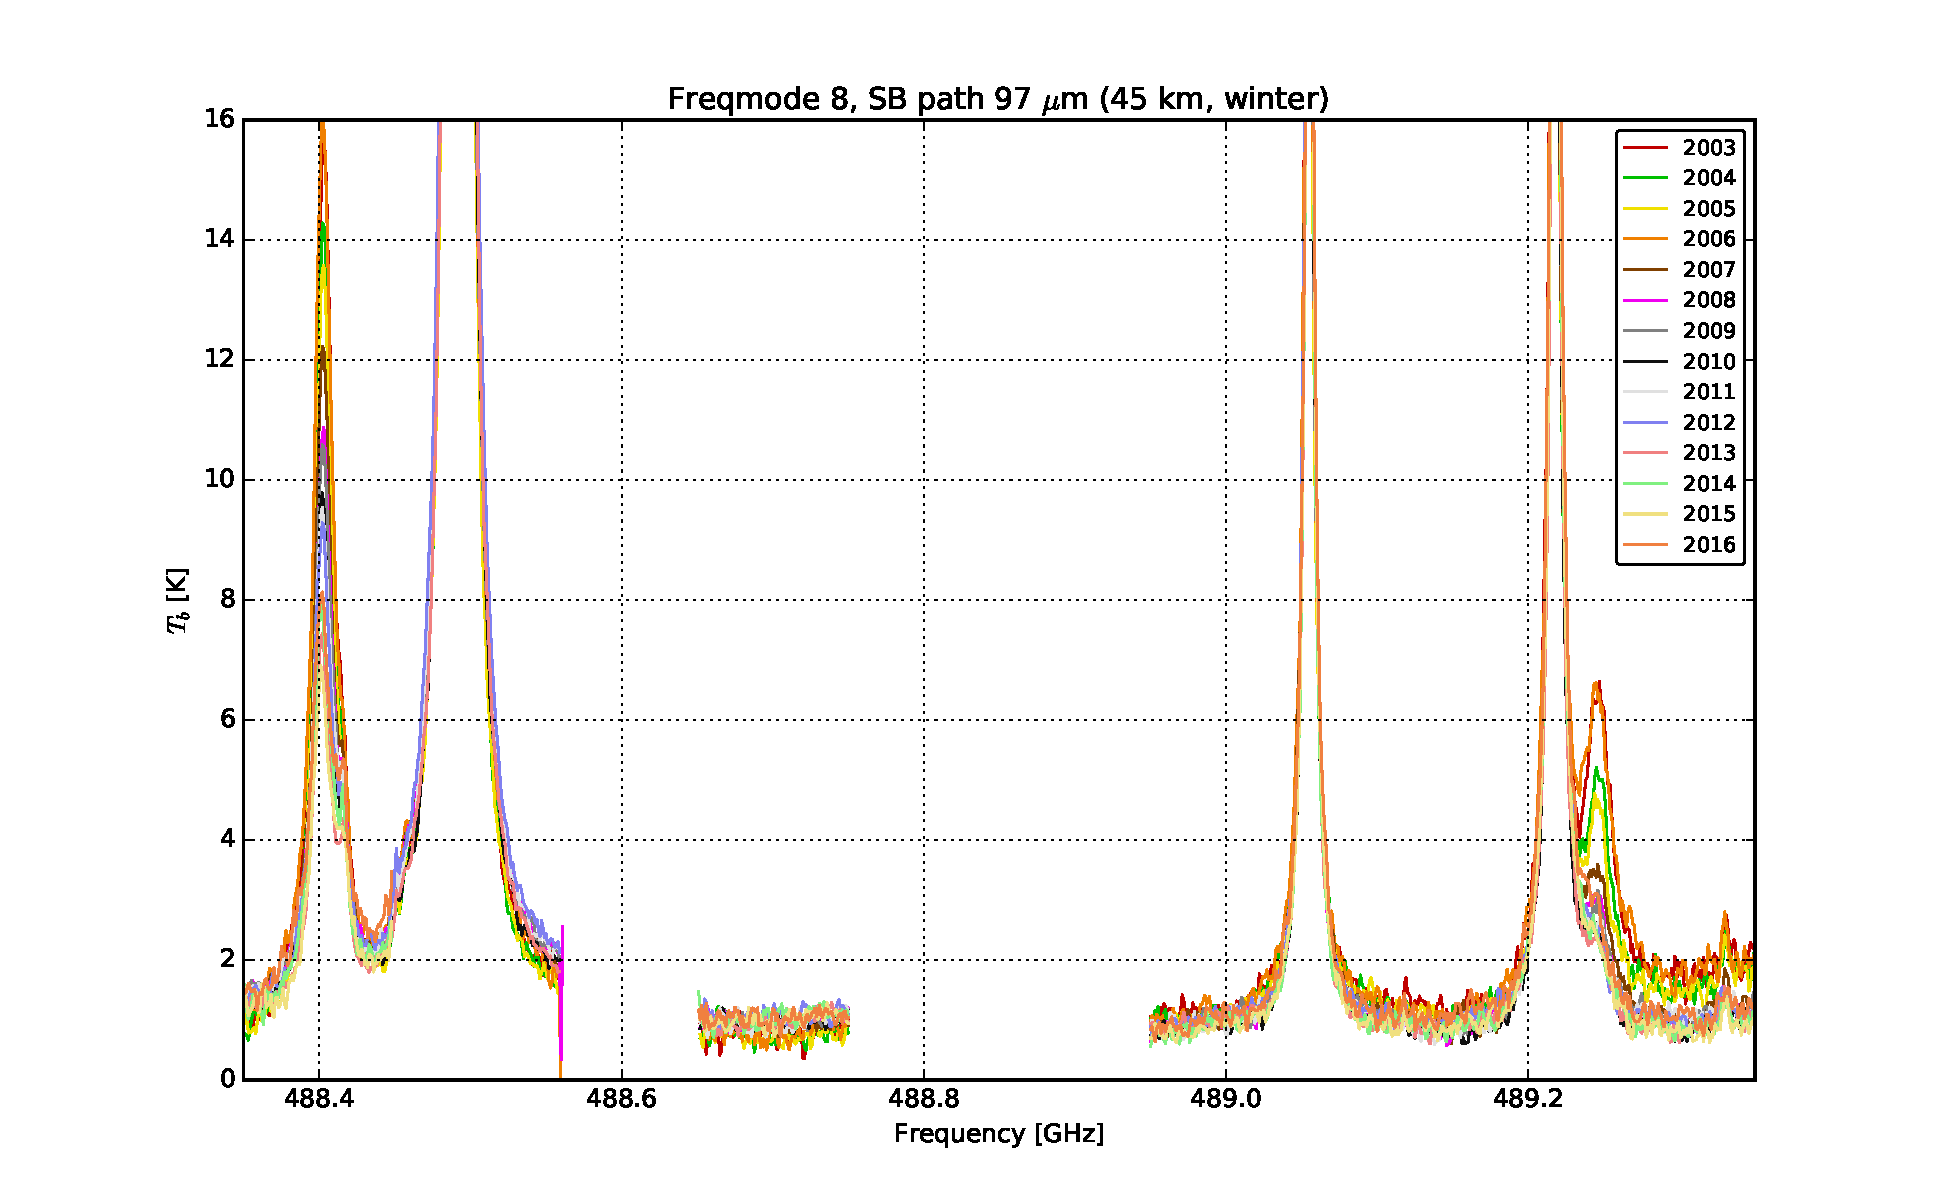
\includegraphics[width=\textwidth]{fm_08_spectra_winter_97u}
        \caption{winter}\label{fig:spectra:08:winter:97u}
    \end{subfigure}
    \caption{Annual median spectra for FM~08 for altitude interval 40--50~km at
        equatorial latitudes for the $97\,\mathrm{\mu m}$ sideband path. The
        unhealthy sub-bands~7 and~3 are between $\sim488.45$
        and~$488.65\,\mathrm{GHz}$.
        }\label{fig:spectra:08:97u}
\end{figure}

\begin{figure}[ht]
    \centering
    \begin{subfigure}[b]{0.9545\textwidth}
        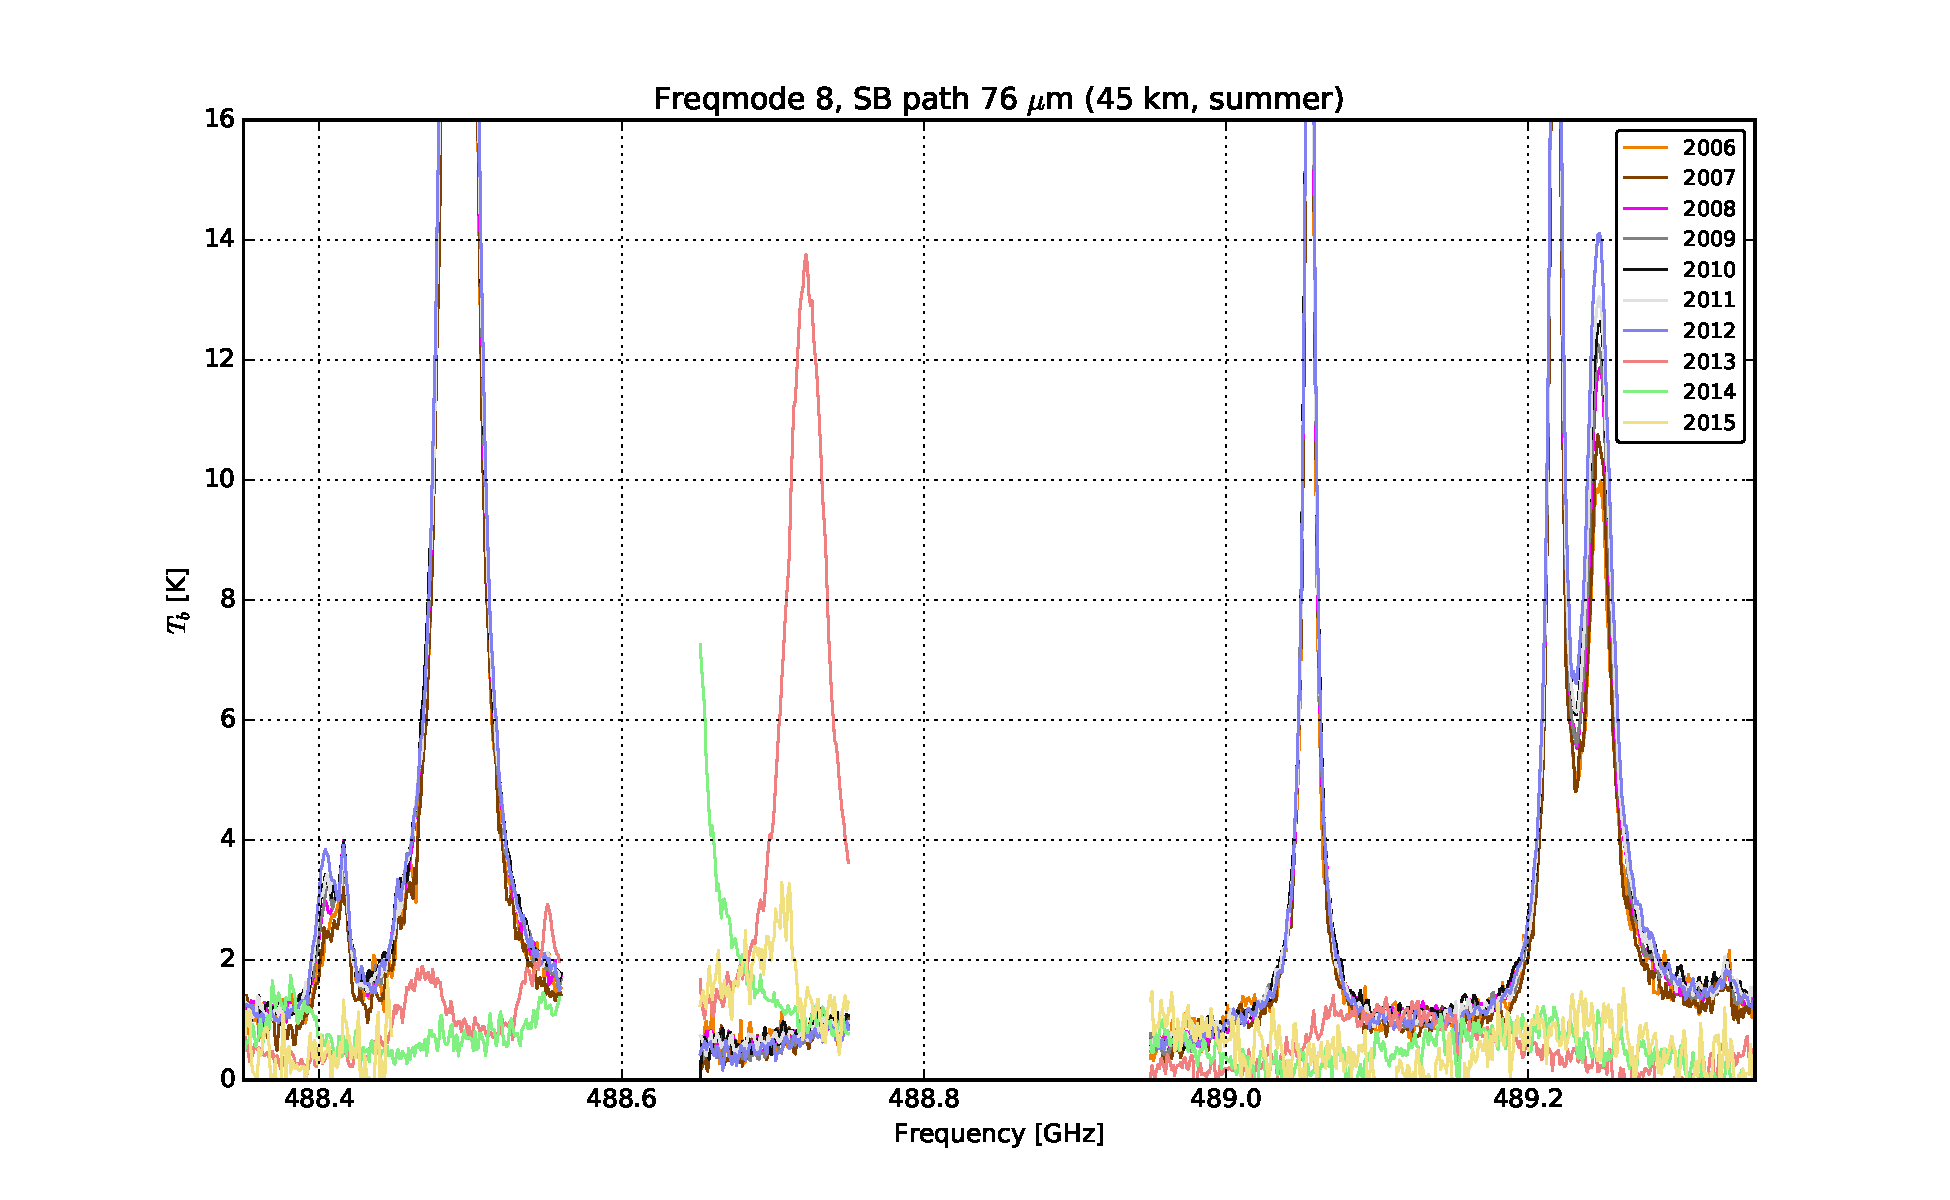
\includegraphics[width=\textwidth]{fm_08_spectra_summer_76u}
        \caption{summer}\label{fig:spectra:08:summer:76u}
    \end{subfigure}
    \begin{subfigure}[b]{0.9545\textwidth}
        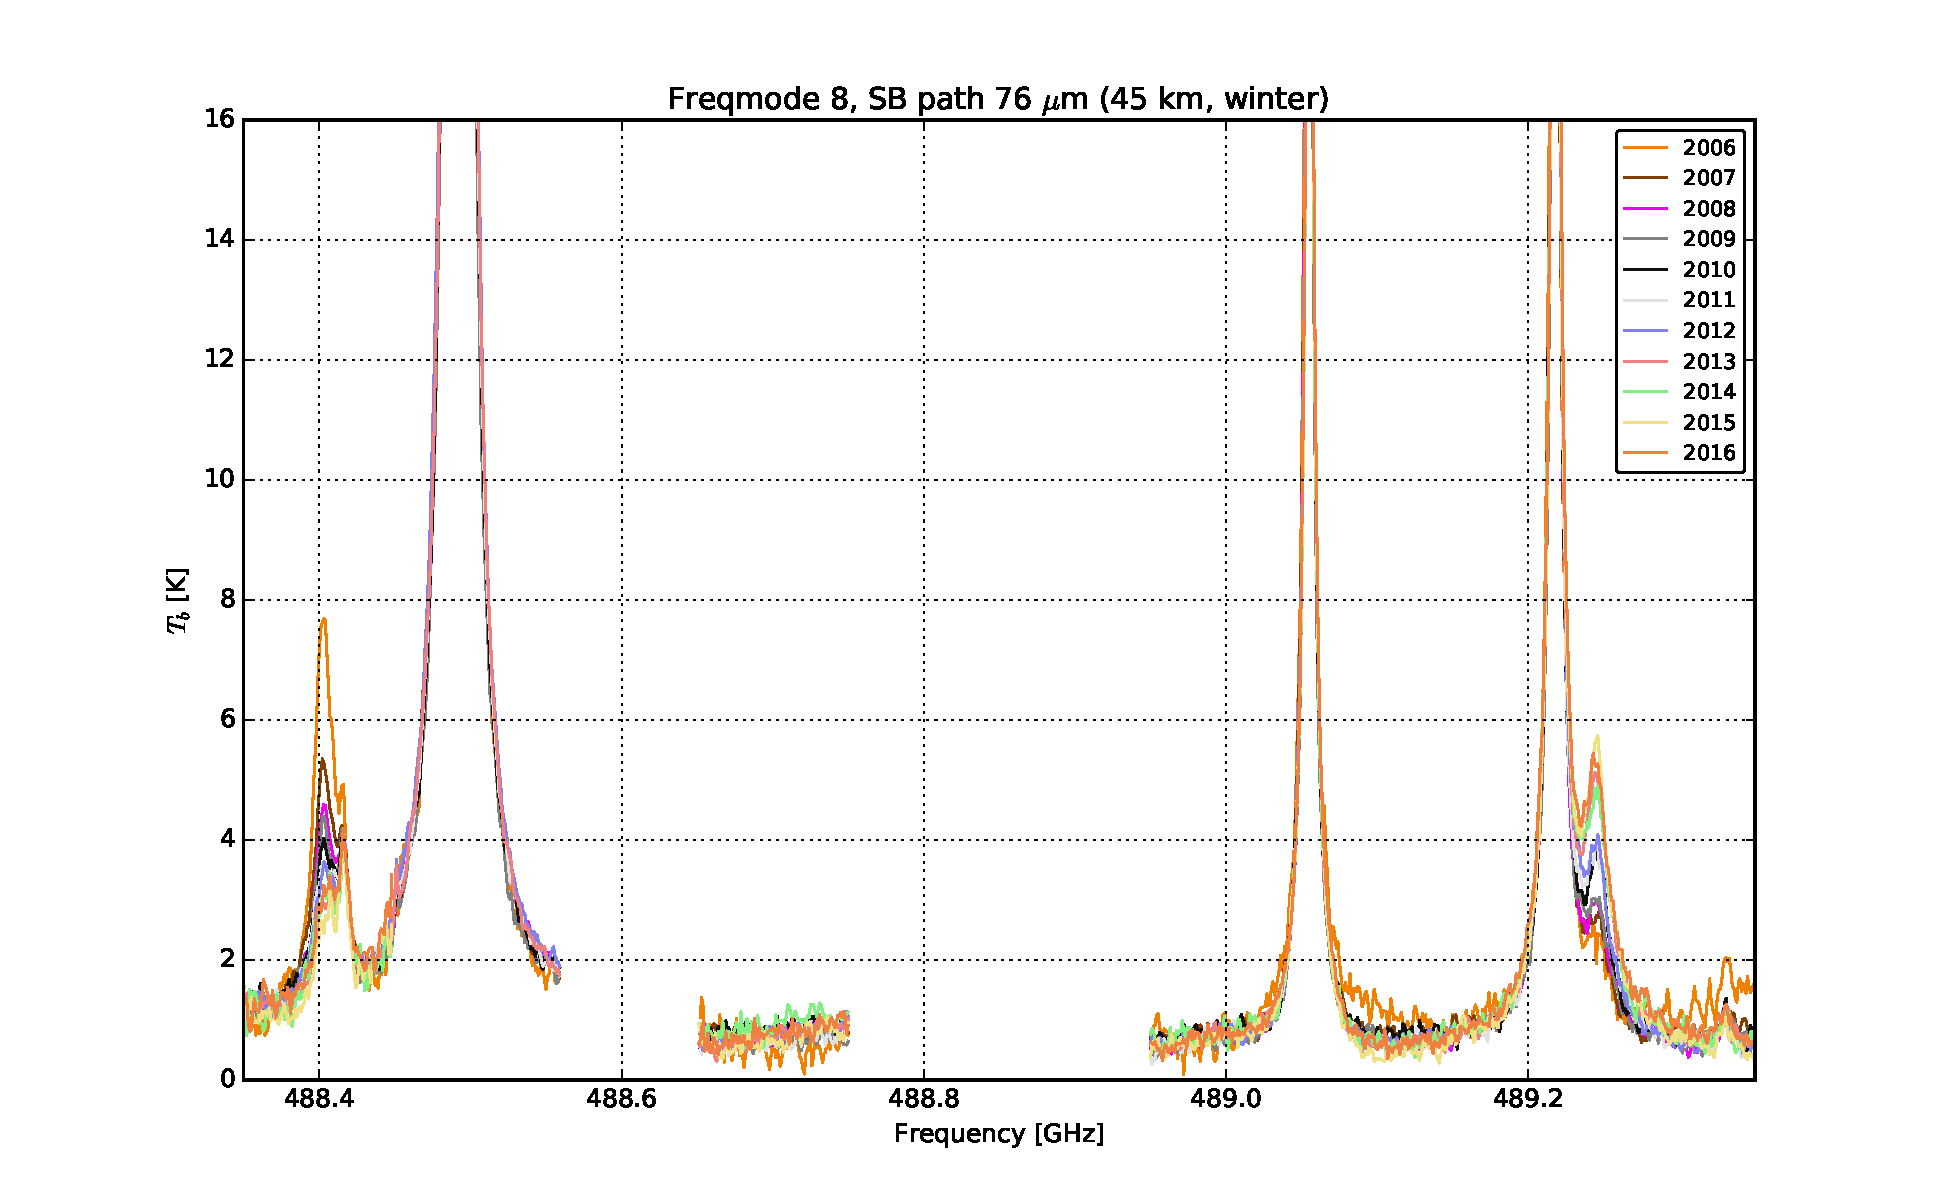
\includegraphics[width=\textwidth]{fm_08_spectra_winter_76u}
        \caption{winter}\label{fig:spectra:08:winter:76u}
    \end{subfigure}
    \caption{Annual median spectra for FM~08 for altitude interval 40--50~km at
        equatorial latitudes for the $76\,\mathrm{\mu m}$ sideband path. The
        unhealthy sub-bands~7 and~3 are between $\sim488.45$
        and~$488.65\,\mathrm{GHz}$.
        }\label{fig:spectra:08:76u}
\end{figure}

\subsection{Sideband leakage}

\begin{figure}[ht]
    \centering
    \begin{subfigure}[b]{0.9545\textwidth}
        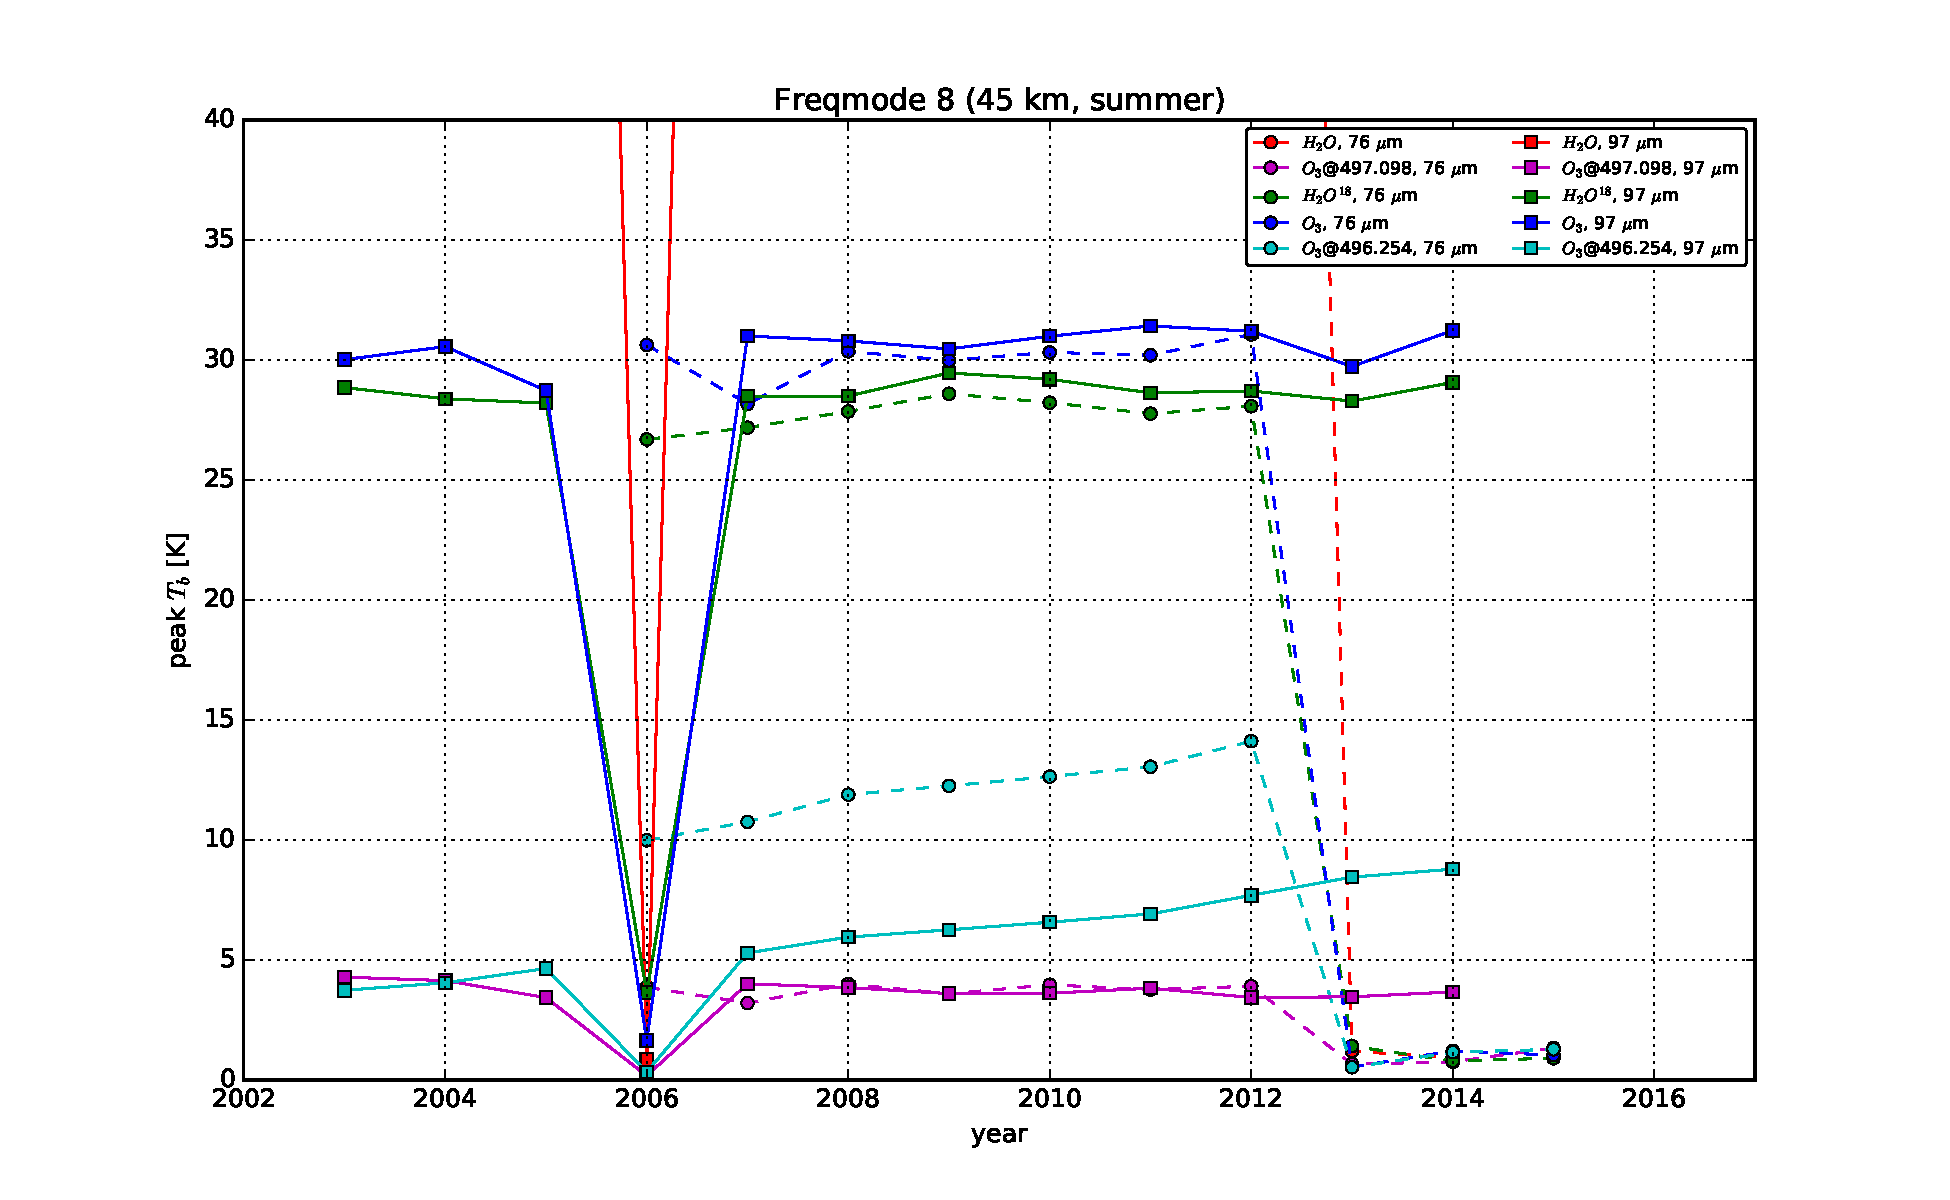
\includegraphics[width=\textwidth]{fm_08_peaks_summer_zoom}
        \caption{summer}\label{fig:peaks:08:summer}
    \end{subfigure}
    \begin{subfigure}[b]{0.9545\textwidth}
        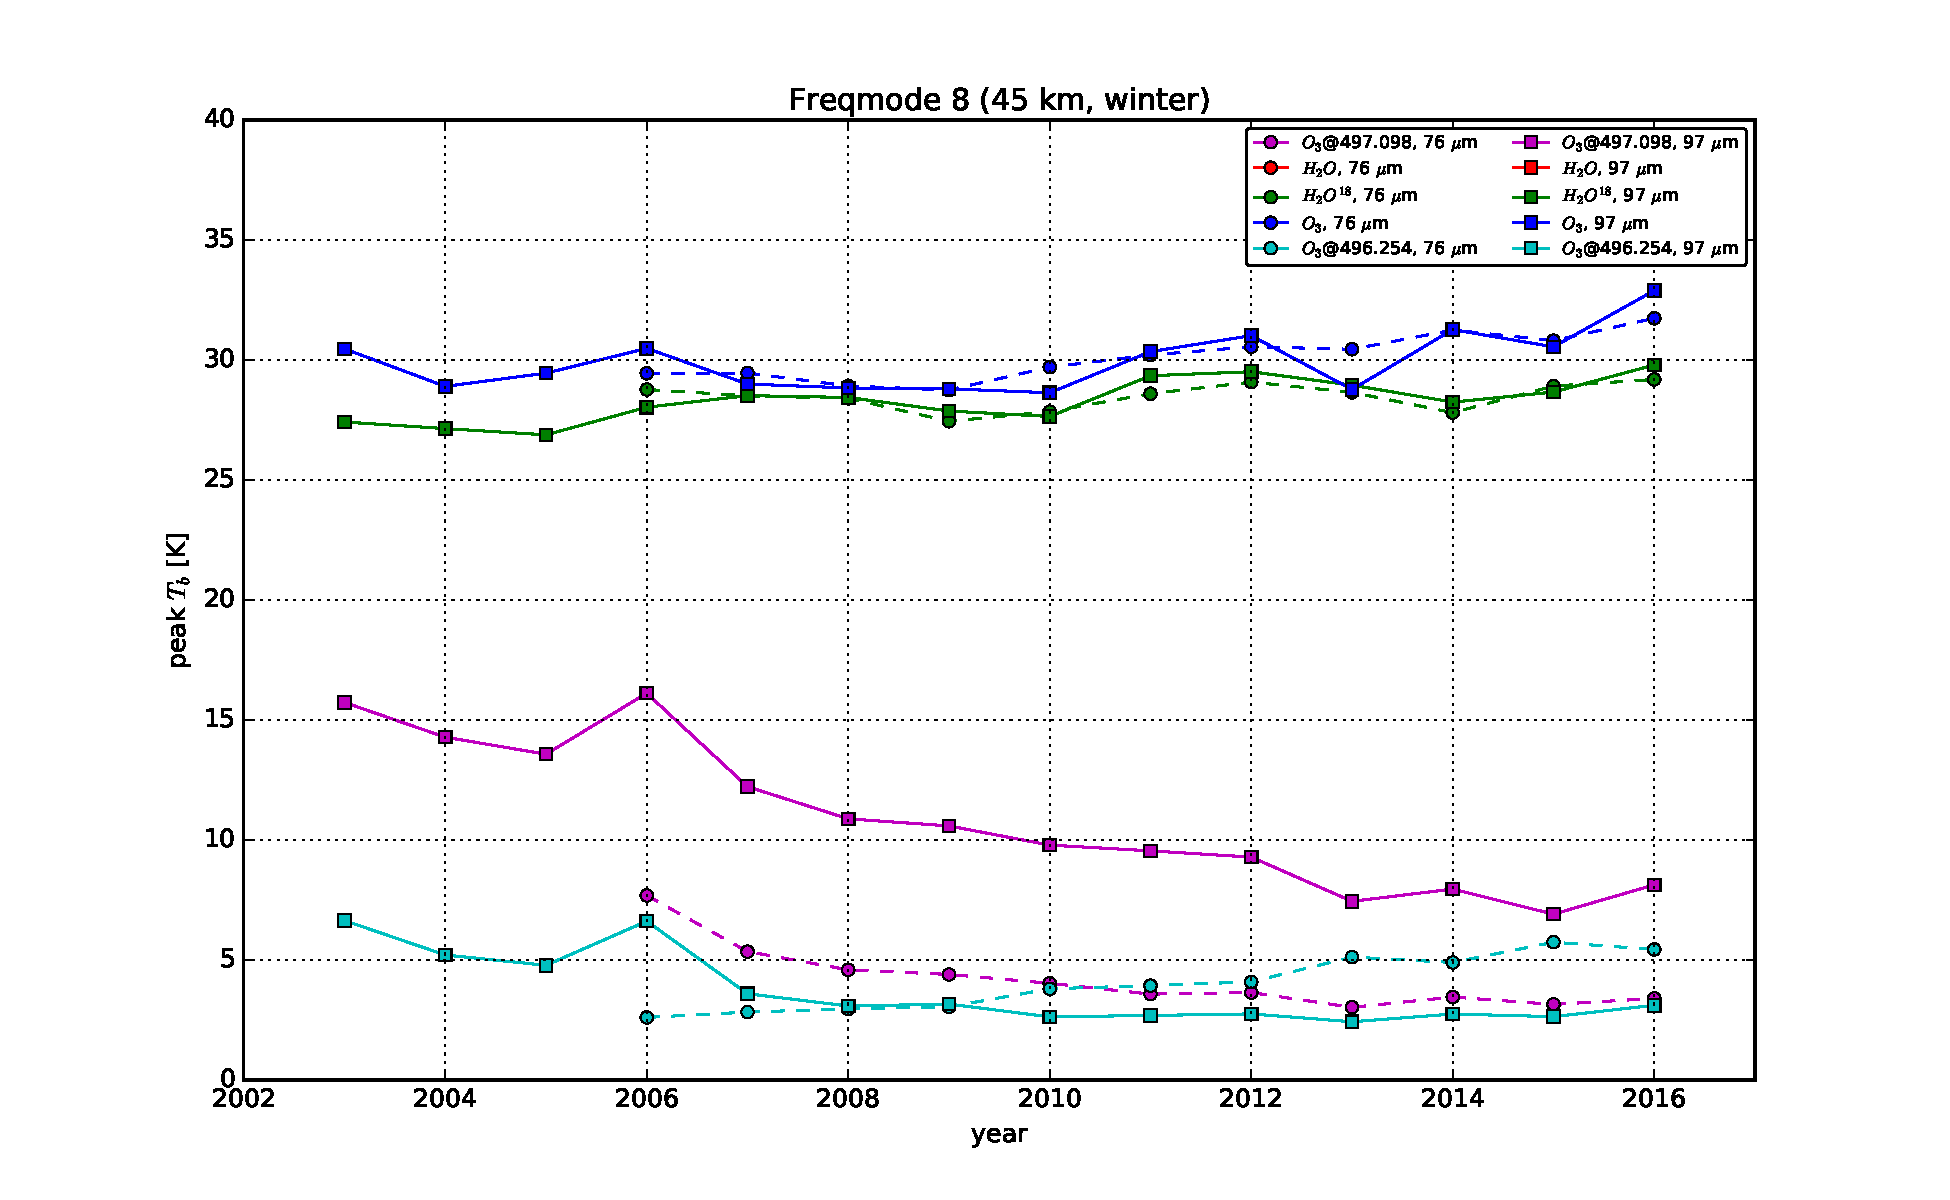
\includegraphics[width=\textwidth]{fm_08_peaks_winter_zoom}
        \caption{winter}\label{fig:peaks:08:winter}
    \end{subfigure}
    \caption{Annual median peak values for FM~08 for altitude interval
        40--50~km at equatorial latitudes for both sideband paths.
        Values extracted for the the \chem{H_2O^{18}} peak
        at~$\sim489.055\,\mathrm{GHz}$, the \chem{O_3} peak
        at~$\sim489.218\,\mathrm{GHz}$, and the \chem{O_3} sideband peaks
        at~$\sim488.405$ and $\sim489.247\,\mathrm{GHz}$,
        in Figs.~\ref{fig:spectra:08:97u} and~\ref{fig:spectra:08:76u}.
        Values were als extracted for the \chem{H_2O} peak
        at~$\sim488.494\,\mathrm{GHz}$, but these are not show due to their
        magnitude.
        }\label{fig:peaks:08}
\end{figure}

\subsubsection{Sideband paths}

\subsection{Seasonality}

